
% \section{Methods of signal reconstruction}
\section{KIDs photometry}
\label{sec:signal}

A dedicated KID readout system has been developed by
\citet{2013A&A...551L..12C} and successfully used for \nika\ and
\nika2\ \todo{which paper should we cite here, all ?}. We here summarize its
main characteristics and the observables that are
relevant for our simulation work. We then present two ways to use them to derive photometry.

%% To convert the $\I(t)$ and $\Q(t)$ that
%% describe the resonance frequency shift $\delta f_0$ to the absorbed optical
%% power $\delta P_{opt}$. We have devised two ways to relate these
%% quantities. Both rely on a specific electronic modulation readout devised by
%% \citet{2013A&A...551L..12C} that we summarize first.

\subsection{Modulated readout technique}
The excitation tone frequency of a KID is modulated by a local oscillator with a
known frequency shift. This provides two values $f_{\pm} = f_0 \pm \frac{\delta
  f_{LO}}{2}$ with $\delta f_{LO} \simeq 1$\,kHz. The ``In-phase'' in
``in-Quadrature'' amplitudes $\I(t)$ and $\Q(t)$ then read:

\begin{equation}
(\I(t), \Q(t)) = (\frac{\I(f_{+}) +
    \I(f_{-})}{2},
\frac{\Q(f_{+}) + \Q(f_{-})}{2}),
\end{equation}

and the differential values are :

\begin{equation}
\label{gradient}
(\di(t), \dq(t)) =
(\frac{\I(f_{+}) - \I(f_{-})}{\delta f_{LO}},
\frac{\Q(f_{+}) - \Q(f_{-})}{\delta f_{LO}}).
\end{equation}

\begin{figure}[h]
\center
	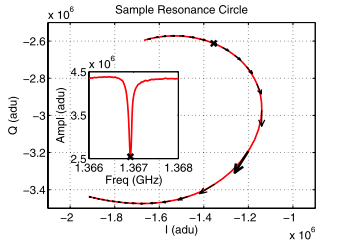
\includegraphics[scale=0.8]{Figures/resonance-circle.png}
	\caption{Representation in the $\I$ - $\Q$ plane of a
          frequency sweep around a resonance. The red line represents the
          $(I,Q)$ data of the frequency sweep around the resonance. The arrows
          represent $(\di, \dq)$. \citep{2013A&A...551L..12C}}
	\label{circle-iq}
\end{figure}

Fig. \ref{circle-iq} shows a typical KID resonance circle. Thanks to this
modulation technique, we obtain four quantities : $\I$ , $\Q$ and their
variation $\di$, $\dq$. In this paper, $\I(t)$ and $\Q(t)$ are sampled at
22\,Hz. They are the mean values over 40 points of $i(t)$ and $q(t)$ that are
sampled at 880\,Hz. $\di(t)$ and $\di(t)$ are the mean values of the difference
between the data measured at $f_{-}$ and $f_{+}$ : \todo{cross check $\di$ vs
  $\delta \I$, $\I(t)$ vs $i(t)$}

\begin{eqnarray}
\I  &=& \sum^{N_{m}=40}_{p=1} i_{p},\\
%\label{eq:i}
\Q  &=& \sum^{N_{m}=40}_{p=1} q_{p},\\
%\label{eq:q}
d\I &=& \sum^{N_{m}/2=20}_{p=1} i_{2p} - i_{2p-1},\\
d\Q &=& \sum^{N_{m}/2=20}_{p=1} q_{2p} - q_{2p-1},
\end{eqnarray}

% on voit les equations \ref{eq:i}, \ref{eq:q}.\\

With these quantities in hand we have several ways to derive the transmitted
signal. They are presented in the following paragraph.

\subsection{\rf}
If a variation $\Delta\I(t)$, $\Delta\Q(t)$ is observed between successive ($\I$,
$\Q$) points, it is possible to estimate the shift of the resonant frequency
$\Delta f_{0}$ between these two samples by comparing ($\Delta \I$, $\Delta \Q$)
with the gradient $(\di,\dq)$ induced by the known $\delta
f_{0}$ of the local oscillator. This is done by a scalar projection of ($\Delta\I$,
$\Delta\Q$) on $(\di,\dq)$ that is tangent to the resonance circle. To have a
cleaner estimation of the latter, we take its average over 50
points that we write $\langle . \rangle_{50}$ \citep{2014A&A...569A...9C}:

\begin{equation}
\label{eq:Rf}
\Delta f_{0} = \delta f_{LO} \frac{\Delta \I\, \langle \di
  \rangle_{50}
+ \Delta \Q\, \langle \dq \rangle_{50}}{\langle \di
  \rangle_{50}^{2}
 + \langle \dq \rangle_{50}^{2}},
\end{equation}

%\delta f_{LO} \frac{\Delta I <dI>_{50} + \Delta Q <dQ>_{50}}{<dI>_{50}^{2} + <dQ>_{50}^{2}}

%% where $\langle . \rangle_{50}$ means that we average the considered quantities
%% over 50 points before and after the concerned value, and $\delta f_{LO} \simeq
%% 1$\,kHz.

This method has been successfully used in \todo{XXXX}, but can be affected by
some systematic uncertainty and be a source of non-linearity. Indeed,
$(\di,\dq)$ is tangent to the $(\I,\Q)$ circle for a fixed background optical
power, while, in principle, the incident optical power that induces the
observable $(\Delta \I, \Delta \Q)$ should distort the resonance circle to some
extent. As a consequence, the observed $(\I,\Q)$ trajectory is not precisely
parallel to the $(\di,\dq)$ direction. Early laboratory and on-site tests have
shown that this approximaton leads to a reconstruction of point source fluxes
better than 2\% \citep{2013A&A...551L..12C}. In this work, we improve this upper
limit on simulations and assess the impact of this error on futures CMB
polarization measurements.

\subsection{Circle fit : Cf}
To improve \rf, we developed a new technique that fully exploits the circular
nature of the $(\I,\Q)$ trajectory, called \cf\ hereafter. The idea of this
method is to project $\I$, $\Q$, $d\I$, $d\Q$, onto an axis $y'$ which is
as linear as possible with frequency and thus with the incident optical
power. Let's denote $Z = \I + j\Q$, near the resonance circle we have:

\begin{equation}
f - f_{0}= \frac{w}{2} \tan \frac{\phi}{2}.
\label{eq:hyp-f}
\end{equation}

\todo{what are $w$ and $\phi$?}\\
The idea is to construct $y'$ from a circle $Z$. The inverse of $Z$ is a circle
but we can normalize it to transform it into an infinite radius circle that is
expected to be linear with the KID frequency.  To do so we define a reference
circle which is centered on ($\frac{1}{2},0$) and has a radius of $\frac{1}{2}$,
after using trigonometric relations we obtain :

\begin{equation}
Z_{ref} = \cos \frac{\phi}{2} e^{j \phi/2}.
\label{eq:Zref}
\end{equation}

If we inverse Eq.~(\ref{eq:Zref}), we have : 
\begin{equation}
Z_{res} = 1 - j \tan \frac{\phi}{2}.
\label{eq:Zres}
\end{equation}

The imaginary part of Eq.~(\ref{eq:Zres}) is linearly dependant on the frequency
defined in Eq.~(\ref{eq:hyp-f}), and represents the new axis $y'$.

From the KID model we have $Z=\I+j\Q$. We do a series of transformations on this
circle to make it identical to the reference circle, the final result is named
$Z'$, with $Z'=p[ZM_{r} + T]$. p is the scaling factor, T represents the
translation and $M_{r}$ is the rotation matrix :

\begin{equation}
M_{r} = 
\begin{pmatrix}
	\cos \alpha & \sin \alpha \\
	-\sin \alpha & \cos \alpha
\end{pmatrix} .
\end{equation}


First we rotate $Z$ :
\begin{equation}
Z' = 
\begin{pmatrix}
	\cos \alpha & \sin \alpha \\
	-\sin \alpha & \cos \alpha
\end{pmatrix}
\begin{pmatrix}
	\I\\
	\Q
\end{pmatrix}
=
\begin{pmatrix}
	\I\cos \alpha + \Q\sin \alpha\\
  - \I\sin \alpha + \Q\cos \alpha
\end{pmatrix}.
\end{equation}

Then we translate and rescale it, to obtain $Z'=\I'+j\Q'$ with : 
\begin{eqnarray}
\I' &=& \frac{1}{2r}[(\I-x_{c}) \cos \alpha + (\Q - y_{c}) \sin \alpha] + \frac{1}{2}, \\
\Q' &=& \frac{1}{2r}[-(\I-x_{c}) \sin \alpha + (\Q - y_{c}) \cos \alpha]. \\
\end{eqnarray}

($x_{c}, y_{c}$), r and $\alpha$ respectively, the center, radius and rotation
angle of the initial circle. The derivative of the inverse of $Z'$ is
$dZ_{res}=-dZ'/Z'^{2}$, with :

\begin{eqnarray}
dZ' &=& d\I' + jd\Q',\\
d\I' &=& -\frac{1}{2r}(d\I \cos \alpha + d\Q \sin \alpha), \\
d\Q' &=& \frac{1}{2r}(-d\I \sin \alpha + d\Q \cos \alpha).
\end{eqnarray}

The imaginary part of $Z_{res}$ and $dZ_{res}$ represent respectively $y'$ and
$dy'$ which are proportional to the KID frequency. We can use these quantities
to calibrate $y'$ and derive the frequency of the KID. In fact, according to the
hypothesis in Eq.~(\ref{eq:hyp-f}), $f$ is a polynomial, so to reconstruct the
shift of the resonant frequency we can fit $\frac{\Delta f}{dy_{3}} = R_{n}(y')$
by a polynomial function, where $R_{n}$ is a polynomial function with a degree
$n$. It is then easy to integrate $R_{n}$ into $P_{n+1}$, with
$\overset{.}{P_{n+1}}=R_{n}$ to obtain the relative frequency of the KID :

\begin{equation}
f - f_{0} = P_{n+1}(y')
\end{equation}

\todo{keep for global conclusion:} In conclusion, because we can not directly
measure the optical power from a KID, new methods were developed to monitor the
shift of the resononance frequency of the detector. First with the modulated
readout technique we can calculate four quantities : $\I$, $\Q$, $\di$,
$\dq$. With these quantities in hand, we can monitor the shift of the resonant
frequency and derive the corresponding incident power ny using the two methods
that were developed : \rf\ which is already successfully used in \nika\ and
\nika2\ (see \citep{2014A&A...569A...9C}) , and \cf\ which is an improvement
from \rf . In this paper, we compare these two methods in terms of linearity. To
do so, in the next sections we do simulations of observations by a KID and we
use \rf\ and \cf\ to reconstruct the signal. We then study the impact of the KID
non-linearity on the search for B modes polarization of the CMB.
